\chapter{Modello dati}
\label{cap:database}
Questo capitolo descrive il database utilizzato all'interno del progetto.\\
Verrà descritto inizialmente la configurazione di Docker, passando per la struttura del database e la gestione dei log nel database.\\

\section{Configurazione di Docker}
I container Docker offrono un'isolamento completo dell'ambiente, che aiuta a evitare conflitti di dipendenze e interferenze con altre applicazioni o servizi che potrebbero essere presenti sul sistema. Per questo motivo si è deciso di utilizzare l'approccio di sandboxing\textsubscript{g} che offre Docker, poichè l'utilizzo di container consente di isolare le applicazioni e i servizi in ambienti virtualizzati, condividendo il kernel del sistema operativo host ma separando le loro risorse e i loro processi.\\
Dato che le tabelle di mia creazione dovevano integrarsi con il database aziendale, tramite il tool Docker Compose e un file di configurazione \textit{docker-compose.yaml}, è stato possibile avviare un nuovo container contenente un'immagine di Microsoft SQL Server, che forniva un backup del database aziendale con dati e tabelle.\\

\section{Progettazione del database}
\subsection{Configurazione di Docker}
I container Docker offrono un'isolamento completo dell'ambiente, che aiuta a evitare conflitti di dipendenze e interferenze con altre applicazioni o servizi che potrebbero essere presenti sul sistema. Per questo motivo si è deciso di utilizzare l'approccio di sandboxing\textsubscript{g} che offre Docker, poichè l'utilizzo di container consente di isolare le applicazioni e i servizi in ambienti virtualizzati, condividendo il kernel del sistema operativo host ma separando le loro risorse e i loro processi.\\
Dato che le tabelle di mia creazione dovevano integrarsi con il database aziendale, tramite il tool Docker Compose\textsubscript{g} e un file di configurazione \textit{docker-compose.yaml}, è stato possibile avviare un nuovo container contenente un'immagine di Microsoft SQL Server, che forniva un backup del database aziendale con dati e tabelle.\\

\subsection{Modello dati}
\textbf{IMMAGINE UML SENZA ATTRIBUTI}\\

\noindent Nel seguente disegno si può notare il database su cui poggia l'API.\\
È stata inserita una nomenclatura <<esterna>> per indicare le tabelle proveniente dal database aziendale.\\
Di seguito elenco le tabelle da me create, spiegandone l'utilizzo e gli attributi:\\

\noindent \textbf{TUTTE LE TABELLE MIE}\\



\section{Gestione dei log nel sistema}
Una tabella di log in un database è una struttura dati che registra le attività che si verificano su una tabella del database. I log sono utili per le seguenti finalità:
\begin{itemize}
\item Sicurezza, possono essere utilizzati per monitorare le attività e gli accessi nel database;
\item Risoluzione dei problemi, possono aiutare gli amministratori del database a capire la radice del problema, facilitando la risoluzione di bug;
\item Recupero dati, ritornano utili in caso di perdita di dati o di necessità a riprendere dati cancellati o modificati;
\end{itemize} 
Per soddisfare il requisito \hyperlink{rf64}{RFDE-64} è stata creata una tabella di log per le Pianificazioni.
Per limiti di tempo non è stata creata e gestita anche l'altra tabella di log delle Richieste come scritto nel requisito \hyperlink{rf46}{RFDE-46}.\\
\subsection{Tabella PianificazioniAudit}
La tabella di log per le Pianificazioni contiene tutti gli attributi di Pianificazioni, ma duplicati. Si distinguono in attributi "old", facendo riferimento ai valori della Pianificazione prima dell'operazione e "new", facendo riferimento ai valori della Pianificazione dopo l'operazione. La chiave primaria della tabella è una chiave composta da: Id della Pianificazione e timestamp dell'attività. Si possono notare anche gli attributi "Utente", per tenere traccia di chi ha effettuato la modifica e l'attributo "Operazione", per indicare se si tratta di un'operazione di cancellazione,inserimento o modifica.\\

\noindent Il popolamento di questa tabella avviene tramite un trigger\textsubscript{g} che si avvia non appena c'è un inserimento, un update o una delete di una riga nella tabella delle Pianificazioni.
\begin{figure}[H] 
    \centering 
    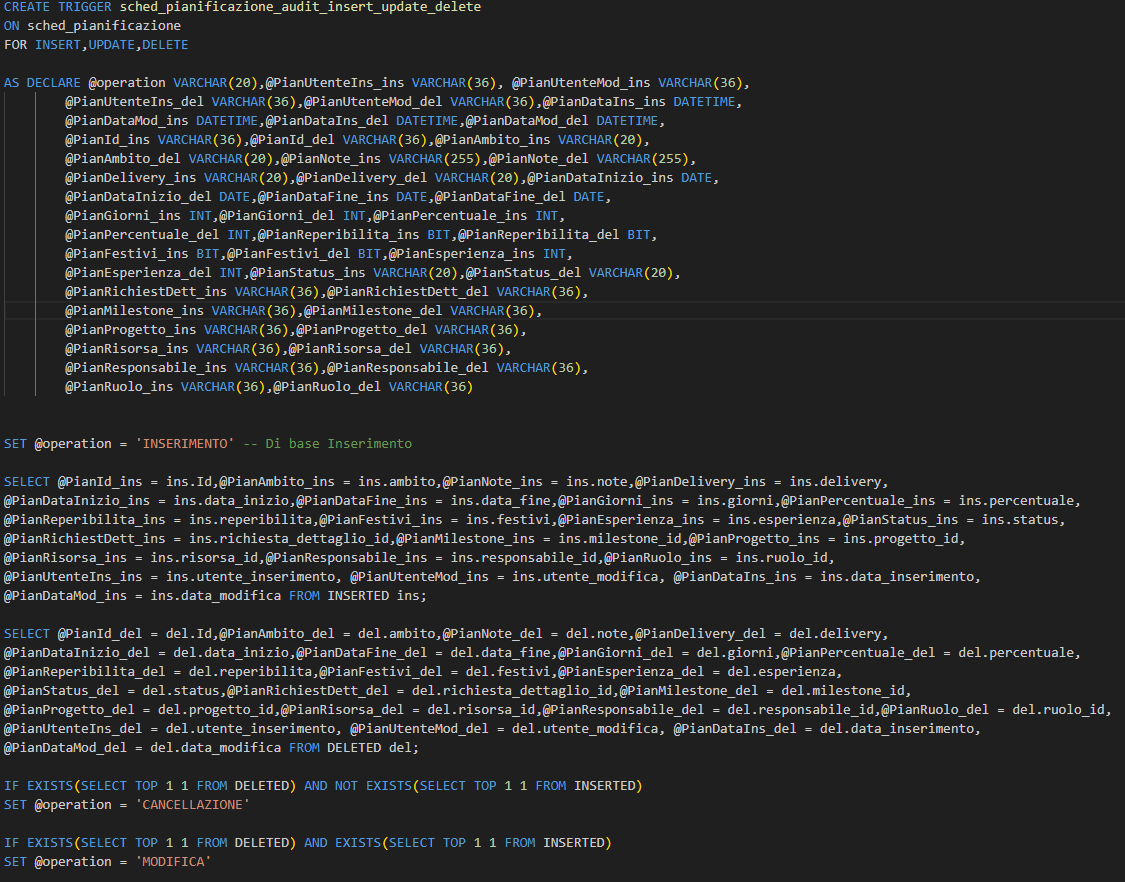
\includegraphics[width=1.0\columnwidth]{trigger-core} 
    \caption{Codice Trigger: Inizializzazione variabili}
\end{figure}

\begin{figure}[H] 
    \centering 
    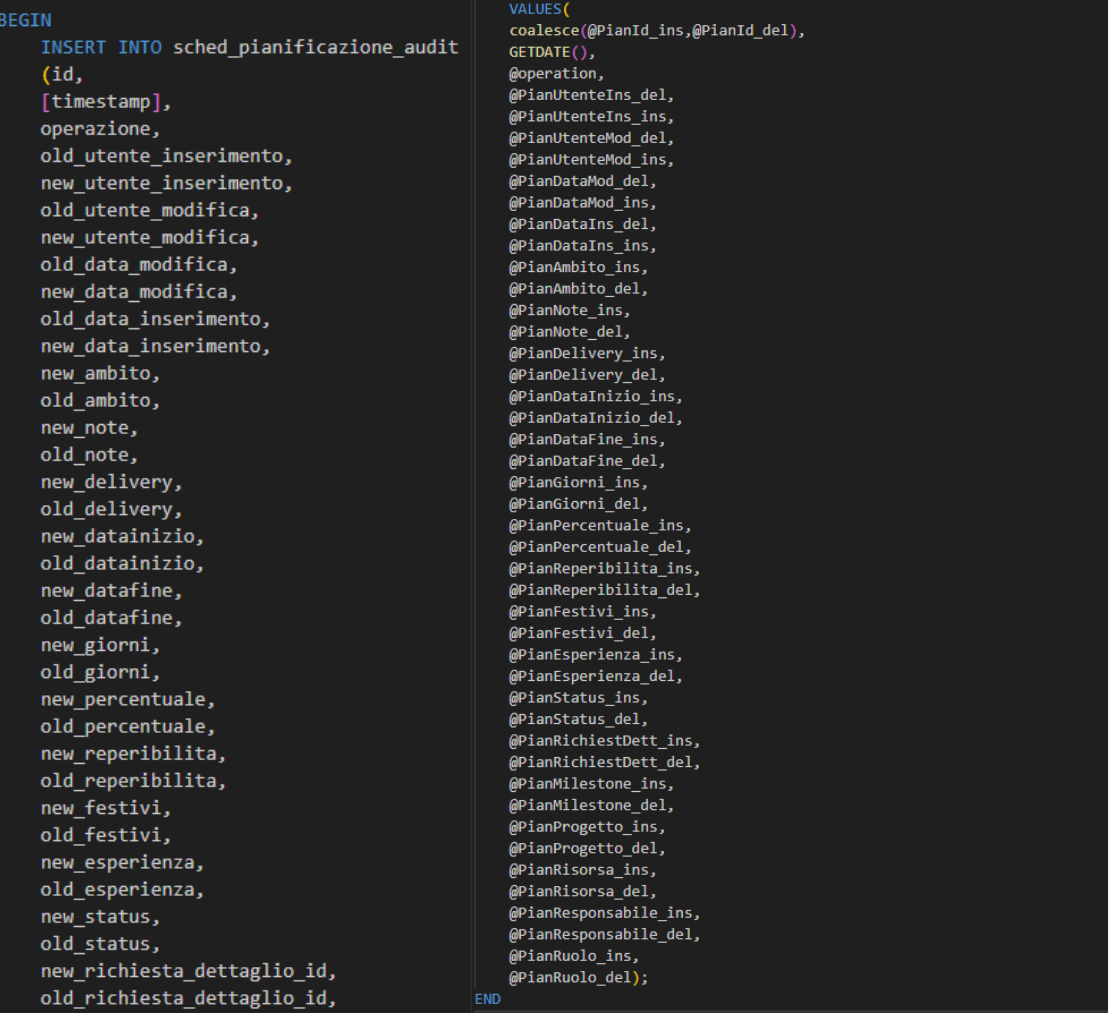
\includegraphics[width=0.8\columnwidth]{trigger-insert} 
    \caption{Codice Trigger: Inserimento dei valori nella tabella di log}
\end{figure}
\noindent Dopo aver definito le variabili, identificato l'operazione effettuata tramite un controllo, vengono eseguiti gli inserimenti nei campi appositi all'interno della tabella.


